\documentclass[11pt]{report}

\usepackage[utf8]{inputenc}
\usepackage{algorithm}
\usepackage{algpseudocode}
\usepackage{hyperref}
\usepackage{graphicx}
\usepackage{subcaption}
\usepackage{booktabs}
\usepackage[square,sort,comma,numbers]{natbib}
\bibliographystyle{abbrv} 

% Title Page
\title{\textbf{A Neural Network to solve square jigsaw puzzles}}
\author{Advanced Machine Learning \\ \\
  Project Report by \\
  Dominique Cheray and Manuel Krämer}

\begin{document}
\maketitle

\tableofcontents

\chapter{Introduction}
\subsubsection*{by Dominique Cheray}
Solving jigsaw puzzles is a pastime that children all over the world know well.
Given a set of often oddly shaped interlocking pieces with small parts of a
picture on top of them the goal is to assemble the pieces in the correct way to
reconstruct the full image. But solving puzzles is not only a fun pastime it
also finds its applications in areas such as archaeology \cite{brown2008system,
  liu2011automated, koller2006computer}, biology
\cite{marande2007mitochondrial}, speech descrambling \cite{zhao2007puzzle},
image editing \cite{cho2008patch} or the reconstruction of fragmented documents
\cite{zhu2008globally}.

The first automatic jigsaw puzzle solvers focus only on the shape of the pieces
to solve the puzzles \cite{freeman1964apictorial, wolfson1988solving,
webster1990computer, kong2001solving}. Later on approaches are presented, which
take into account the color information in addition to the shape of the pieces
\cite{kosiba1994automatic, makridis2006new, sagiroglu2006texture}. Recent work
began to focus on only using the color information of the pieces
\cite{nielsen2008solving} which then eventually shifted to only consider jigsaw
puzzles with square pieces where color information is the only information that
can be used to find matching pieces \cite{Cho2010, yang2011particle,
  Pomeranz2011, gallagher2012jigsaw, son2014solving, sholomon2013genetic,
  Paikin2015, sholomon2016dnn}.

The first to introduce square pieces are Cho et al. \cite{Cho2010}. They present
a probabilistic solver that can handle puzzles of up to 432 pieces. To solve the
puzzle the solver needs some apriori knowledge of the puzzle, namely its size
and the position of few so-called ``anchor-pieces'' which are placed at their
correct location prior to the placement of the remaining pieces. A year later
the results of Cho et al. are improved by Yang et al. \cite{yang2011particle}
which use a particle filter based solver.

Pomeranz et al.\cite{Pomeranz2011} are the first to introduce a fully automatic
jigsaw puzzle solver. Their solver is based on a greedy placer and can handle
puzzles of up to 3,300 pieces. Later on the work of Pomeranz et al. is improved
and extended by both Gallagher et al. \cite{gallagher2012jigsaw} and Son et al.
\cite{son2014solving}. Gallagher use a greedy tree algorithm and generalize the
work of Pomeranz et al. to also handle pieces of unknown orientation and puzzles
with unknown dimensions. Son et al. add ``loop constraints'' to the work of
Gallagher et al. which allows them to handle pieces of unknown orientation.

Instead of a greedy solver Sholomon et al. \cite{sholomon2013genetic} present a
genetic algorithm that is able to solve large square jigsaw puzzles. Later on
they improve their work by introducing a deep neural-network based estimation
metric \cite{sholomon2016dnn}. Given the edges of two pieces the neural network
predicts whether the two pieces belong next to each other in the correctly
assembled puzzle or not. The authors state that their metric shows
extremely high precision without the need of manual feature extraction. When
integrated into an existing solver it will significantly improve the results
\cite{sholomon2016dnn}. 

The solver presented by Paikin \& Tal \cite{Paikin2015} is inspired by the work
of Pomeranz et al. \cite{Pomeranz2011}. Their algorithm is also a greedy solver
but is able to solve more challenging puzzles. It can handle jigsaw puzzles with
missing pieces, pieces of unknown orientation, puzzles of unknown size and
multiple puzzles whose pieces are mixed together. The placement of the puzzle
pieces is based on a compatibility function but they provide a faster and more
accurate function than previous works. Additionally, since early mistakes can
have a fatal impact when using a greedy placer, they take special care when
choosing the first piece to place. Earlier works randomly select the first
piece. Another change made by Paikin \& Tal is to place the pieces in relation
to the pieces already placed and not on absolute positions. So the next piece to
place is not the piece that best fits a particular spot, but the most likely to
be correct.

For this project we will integrate the neural-network based estimation metric
proposed by Sholomon et al. \cite{sholomon2016dnn} in our reimplementation of the
solver by Paikin \& Tal \cite{Paikin2015} from last semester's project. We evaluate the resulting
solver with the same image datasets as the authors and compare our result to
theirs as well as to the results from our implementation of Paikin \& Tal's
solver from last semester.

\chapter{Theoretical Background}
\subsubsection*{by Dominique Cheray}

\chapter{Materials and Methods}
\subsubsection*{by Manuel Krämer}
\section{Algorithm}
\label{sec:algo}
The algorithm we implemented is the one that was used in \cite{Paikin2015} with the extension of a neural network as proposed by \cite{sholomon2016dnn}. The whole procedure can be described by three main steps:
\begin{enumerate}
	\item Compatibility between pieces: This is done by calculating the dissimilarity between two pieces. The so-called "Best Buddies"-metric, which was used by \cite{Paikin2015}, is replaced by the DNN-Buddies that are determined by a Neural Network. This metric indicates, that two pieces agree that each other is their best neighbor.
	\item First piece: As described by \cite{Paikin2015} one important step is to find a good starting piece which has best buddies in all four spatial relations and these four neighbors have best buddies in all directions as well.
	\item Placer: The placing of the pieces is done by grabbing the best piece (highest compatibility) from a pool, placing this piece and adding the best buddies of it to the pool.
\end{enumerate}

\subsection{Compatibility between pieces}
The most fundamental part is the calculation of the compatibility between two pieces to determine how well they fit together. This is done by computing the dissimilarity between every pair of pieces and with this score you can tell if the pieces have similarities or not.

First of all, the dissimilarity of two pieces $p_i$ and $p_j$ is defined as follows (see \cite{sholomon2016dnn}): 
\begin{equation}\label{eq:dissimilarity}
	D(x_i,x_j,right) = \sqrt{\sum_{k=1}^K \sum_{d=1}^3 (p_i(k,K,cb) - p_j(k,1,cb))^2}
\end{equation}
K is the piece size and cb the color band.

\subsection{First piece}
One important task is to avoid early errors because the algorithm considers the unplaced and placed pieces as well. If there is a mistake within the first few pieces this can lead to following errors.
This means we need a first piece that is located in a distinctive area where the probability of making errors is as low as possible. A good measure for this is the DNN-buddies metric. We require the first piece to have best buddies in all four spatial relations, what ensures that the piece itself is distinctive. Furthermore, all four neighbors of this piece need to have best buddies in all four spatial relations as well, what means that the piece is located in a distinctive region. 
Usually, there is more than one piece that satisfies these conditions. Out of all these distinctive pieces we choose the one with the best buddies that maximize the compatibility in all four spatial relations.

\subsection{Placer}
The placer algorithm as described in \cite{Paikin2015} places all pieces according to their compatibility and maintains a pool with potential pieces to place. Since the description is not detailed there are several possibilities to implement it so we want to give a more comprehensive explanation of our method (see algorithm \ref{algo:placer}).

\begin{algorithm}
	\caption{Placer algorithm}
	\label{algo:placer}
	\begin{algorithmic}
		\State Place the first piece into the pool
		\While{There are unplaced pieces}
		\While{Pool is not empty}
		\State Get the best item and its placing position from the pool
		\If{Placing position is occupied}
		\State Delete the piece from processedPieces and continue \EndIf
		\State Add this item to the placer List
		\State Delete this item from unplaced pieces
		\State Save the taken indices
		\State Calculate all best buddies and put them in the pool
		\EndWhile
		\Comment{Pool is empty}
		\State Get best piece of all unplaced
		\If{Placing position is not occupied}
		\State Put this piece on the pool
		\EndIf
		\EndWhile
	\end{algorithmic}
\end{algorithm}

With this approach, we make sure that an already placed piece doesn't get overwritten by pieces that maybe have a high compatibility as well. While processing through all pieces we keep track of the row and column indices of every piece so we can detect duplicates and, finally reconstruct the puzzled image.
\newpage

\section{Neural Net}
The architecture of the neural net is the one proposed by \cite{sholomon2016dnn}. In Figure \ref{fig:NN} one can see that it is a simple 4-layer, fully-connected network which uses the two edge rows/columns of two adjacent pieces as an input. The classification between "best buddy" and "not best buddy" is done by a softmax classifier that produces the probability of the two cases. The activation for all layers is the rectified linear unit (ReLU) function and we trained the network with the Stochastic Gradient Descent.
\begin{figure}[ht]
	\centering
	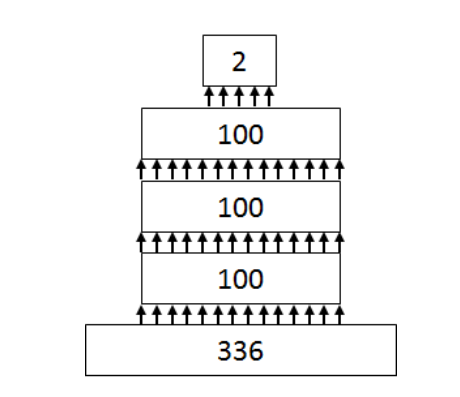
\includegraphics[width=0.6\textwidth]{NeuralNet.PNG}
	
	\caption{The architecture of the neural net (from \cite{sholomon2016dnn})}
	\label{fig:NN}
\end{figure}


\section{Image data and evaluation}
\subsection{Training data of the Neural Net}
For training and cross-validation we use 2218 images from the IAPR TC-12 Benchmark (see \cite{grubinger06}, one can see a sample of those in figure \ref{fig:IAPR-database}). These images have a resolution of 360 $\times$ 480 pixels and we convert them into YUV color space before processing. After normalization the images get cut into 12 $\times$ 17 tiles which are used to produce a training set for the neural network in the following way:
\begin{itemize}
	\item For each puzzle piece edge $x_{i,j}$, find the most compatible piece edge $x_{k1,l1}$ and its second most compatible piece edge $x_{k2,l2}$
	\item  If the pair $x_{i,j}$ - $x_{k1,l1}$ is originally adjacent, add this pair to the positive labeled and the pair $x_{i,j}$ - $x_{k2,l2}$ to the negative labeled
	\item If this is not the case, add $x_{i,j}$ - $x_{k1,l1}$ to the negative labeled and discard the pair $x_{i,j}$ - $x_{k2,l2}$
\end{itemize}
To decide if two pieces are adjacent the most important regions are the edges. So one (positive or negative) instance contains the two edge rows/columns of one piece and two adjacent rows/columns of the other. Since all images from \cite{grubinger06} have the same size the procedure described above results in an image array of 336 pixels (28 pixels $\times$ 4 rows/columns $\times$ 3 color chanels).

\begin{figure}
	\centering
	\begin{subfigure}[b]{0.45\textwidth}
		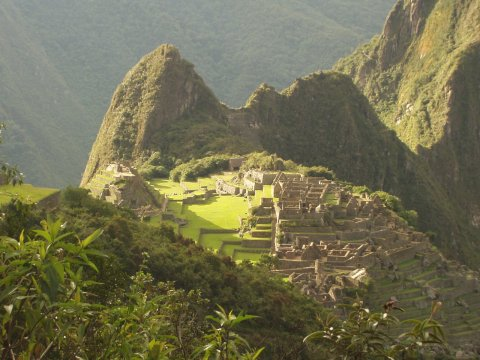
\includegraphics[width=\textwidth]{../iaprtc12/images/24/24019.jpg}
		\caption{One image of the dataset}
		\label{img:432}
	\end{subfigure}
	~
	\begin{subfigure}[b]{0.45\textwidth}
		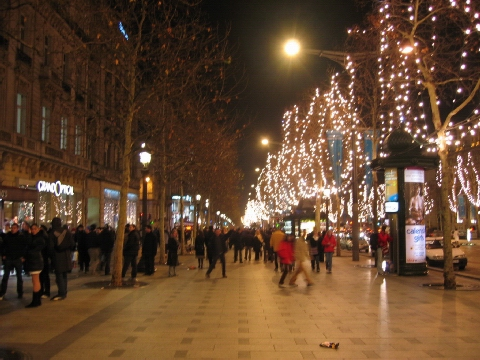
\includegraphics[width=\textwidth]{../iaprtc12/images/37/37142.jpg}
		\caption{Another image of the dataset}
		\label{img:540}
	\end{subfigure}
	
	\caption{A sample of all the datasets we used for the training of the neural net}
	\label{fig:IAPR-database}
\end{figure}

\subsection{Evaluation}
By testing the algorithm we used images from \cite{Cho2010} (size: 432 pieces) and \cite{Pomeranz2011} (size: 540, 805 and 2360 pieces) to get comparable results. A small sample of these data one can see in fig. \ref{fig:database}

\begin{figure}
	\centering
	\begin{subfigure}[b]{0.45\textwidth}
		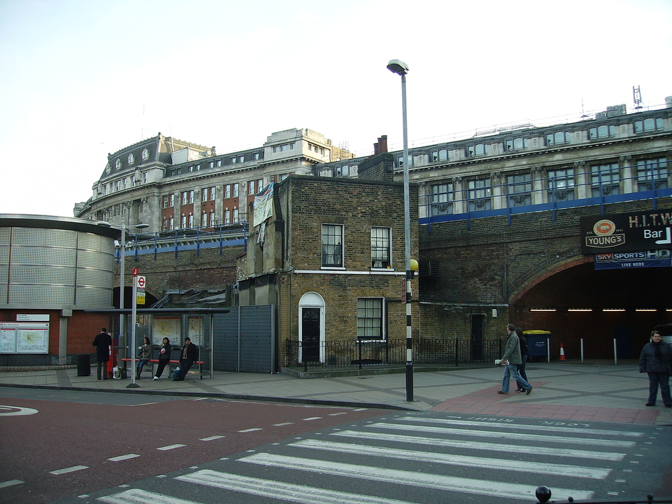
\includegraphics[width=\textwidth]{../imData/432/1.png}
		\caption{One image of the dataset we used for the puzzle with 432 pieces}
		\label{img:432}
	\end{subfigure}
	~
	\begin{subfigure}[b]{0.45\textwidth}
		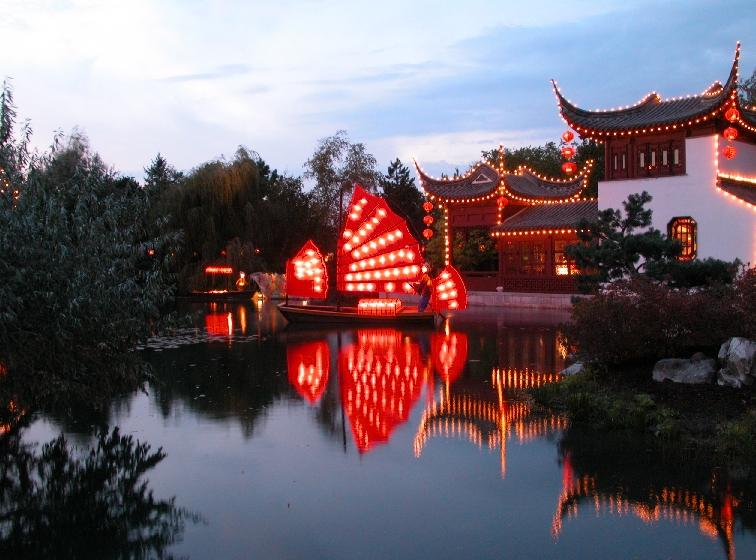
\includegraphics[width=\textwidth]{../imData/540/1.jpg}
		\caption{One image of the dataset we used for the puzzle with 504 pieces}
		\label{img:540}
	\end{subfigure}
	~
	\begin{subfigure}[b]{0.45\textwidth}
		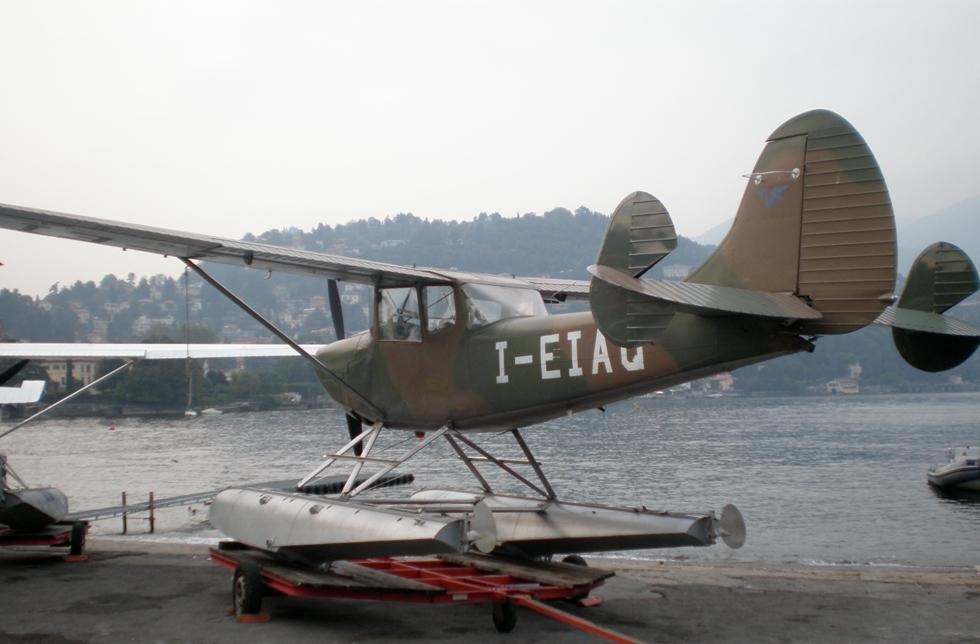
\includegraphics[width=\textwidth]{../imData/805/1.jpg}
		\caption{One image of the dataset we used for the puzzle with 805 pieces}
		\label{img:805}
	\end{subfigure}
	~
	\begin{subfigure}[b]{0.45\textwidth}
		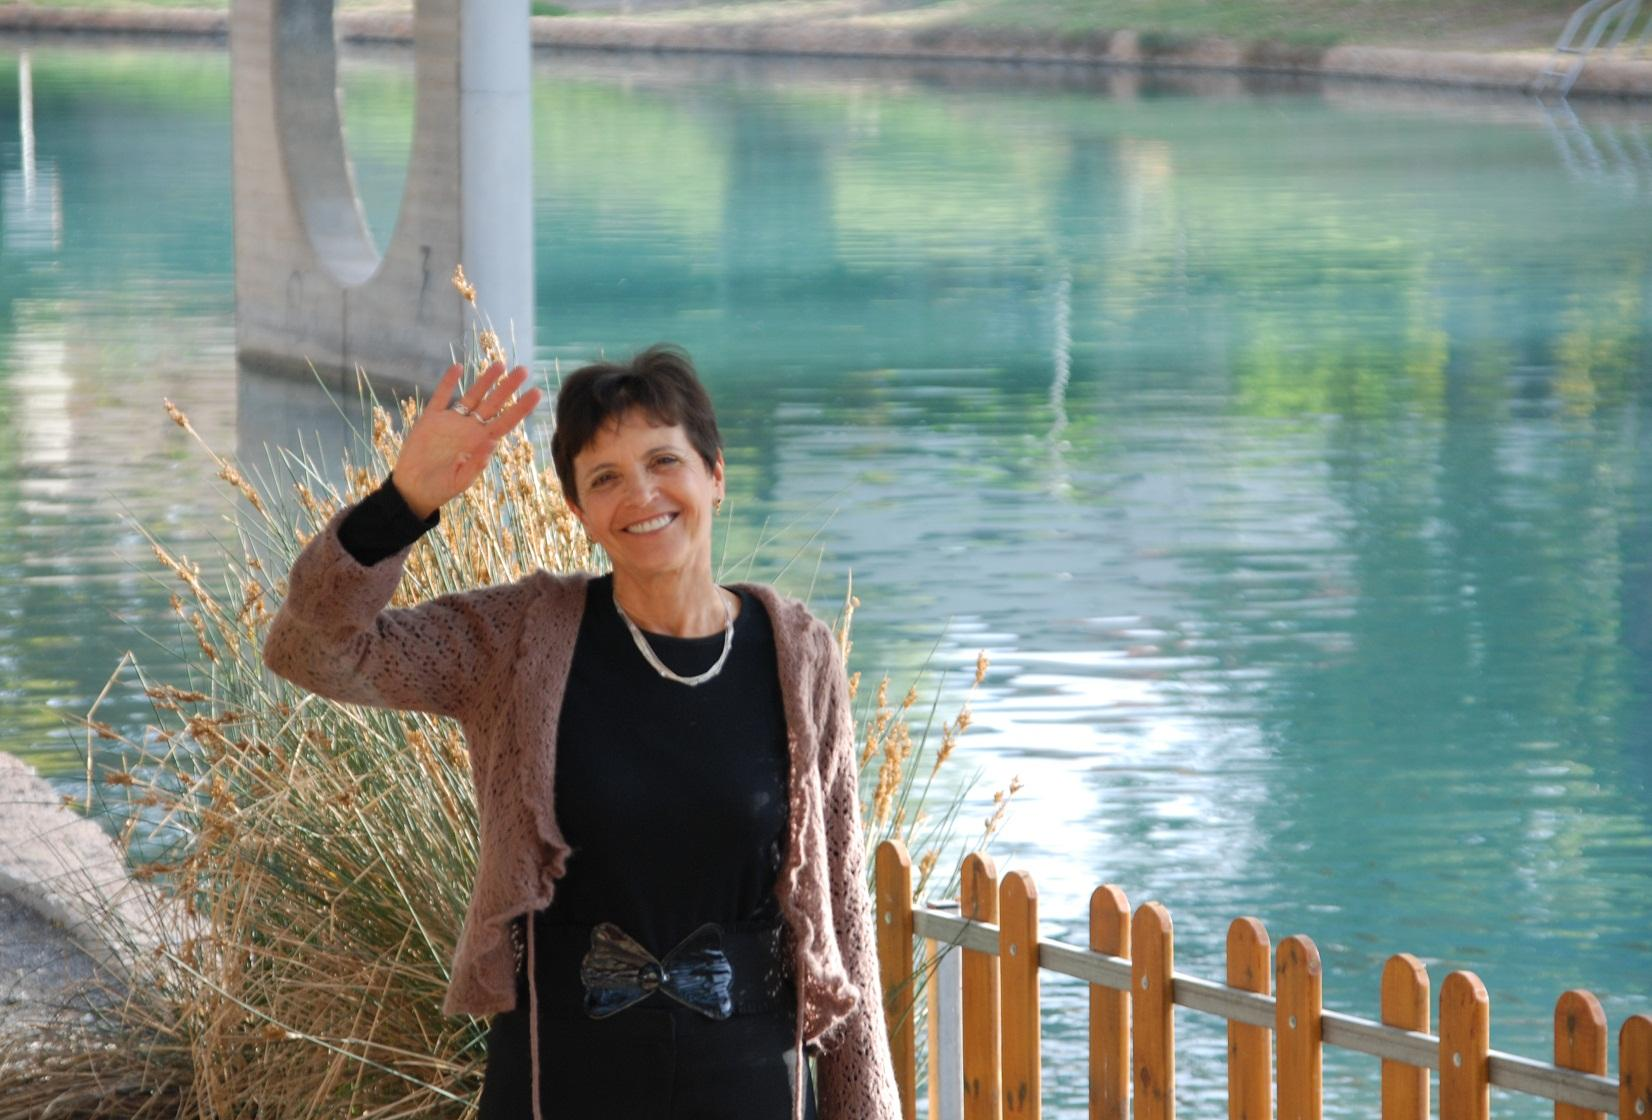
\includegraphics[width=\textwidth]{../imData/2360/1.jpg}
		\caption{One image of the dataset we used for the puzzle with 2360 pieces}
		\label{img:2360}
	\end{subfigure}
	
	\caption{A sample of all the datasets we used for evaluation}
	\label{fig:database}
\end{figure}

To evaluate our results we used the direct measure, i.e. to check the absolute position of every piece in the image and the relative score which determines how many correct neighbors each piece has.


\bibliography{literature}

\end{document}    
